\chapter{IoT}
Sempre più spesso si parla di Internet delle cose, o IOT, con questo termine si 
intende un evoluzione delle applicazioni legate al settore mobile, al settore
della home automation e al settore embedded. 
In questo scenario ogni oggetto il
quale contiene un sensore sarà connesso ad Internet. Avvalendosi di questa
connessione , i vari dati raccolti potranno essere inviati nel cloud, dove
verranno elaborati e resi disponibili alle varie applicazioni. 
Per fare in modo che ciò  avvenga, è necessario riuscire a creare una
rete di devices in grado di  
\textit{parlare un linguaggio comune}. \improvement{Scrivi qualcosa di decente qui}

\begin{tcolorbox}
Il vero valore aggiunto dell'IoT è la possibilità di processare i dati raccolti
direttamente nel cloud utilizzando tecniche di data analytics, per giunta
ogni devices sarà composto da un hardware semplice e conseguentemente il costo
unitario sarà molto basso.
\end{tcolorbox}

Come già succede per le applicazioni embedded, da un decennio a questa parte,
anche nel IoT è il software il vero valore aggiunto, nel caso specifico i dati
che i vari sensori raccolgono. Riuscendo ad inviare il dato raccolto
direttamente ad un server, si ha la possibilità di implementare hardware
semplice al interno dei vari dispositivi, lasciando l'elaborazione del dato
direttamente al server tramite tecniche di data analytics.

\begin{tcolorbox}
Avendo la possibilità di processare i dati raccolti
direttamente nel cloud utilizzando tecniche di data analytics, il dato in se
diventa il valore aggiunto del IoT. Spostando la concentrazione da hardware a
software,  ogni devices sarà composto da un hardware semplice e conseguentemente il costo
unitario sarà molto basso.
Spostando il vero valore dal hardware al \emph{dato}, è necessario disporre di
tecniche buone per il data analytics

Come successo agli albori di Internet, anche nel IoT, siamo in presenza di
diversi standard per il tipo di comunicazione da adottare.
Il punto principale di questo
upgrade sta nel riuscire a creare una rete di devices connessi ad internet. Per
supportare e utilizzare una potenza di calcolo maggiore andando a combinare
tecniche di data analytics per estrarre le informazioni più significative. 
\end{tcolorbox}

In questa visione, milioni di devices saranno connessi a Internet e molto presto
milioni di milioni di devices. 

Il mercato di questi \emph{smart devices } è
in rapida crescita con una stima di 8,3 miliardi di dispositivi connessi nel
anno 2017, e di circa 20 miliardi per l'anno 2020 \cite{gartner2016}. Andando ad
creare un impatto economico compreso tra i 2.7 e i 14 trilioni di dollari. I
mercati principali saranno quelli del healt care con un introito compreso tra i
$1.1$ e i $2.5$ trilioni di dollari e il settore industriale con $2.3$ a $11.6$
trilioni di dollari.

\begin{figure}[h]
\centering 
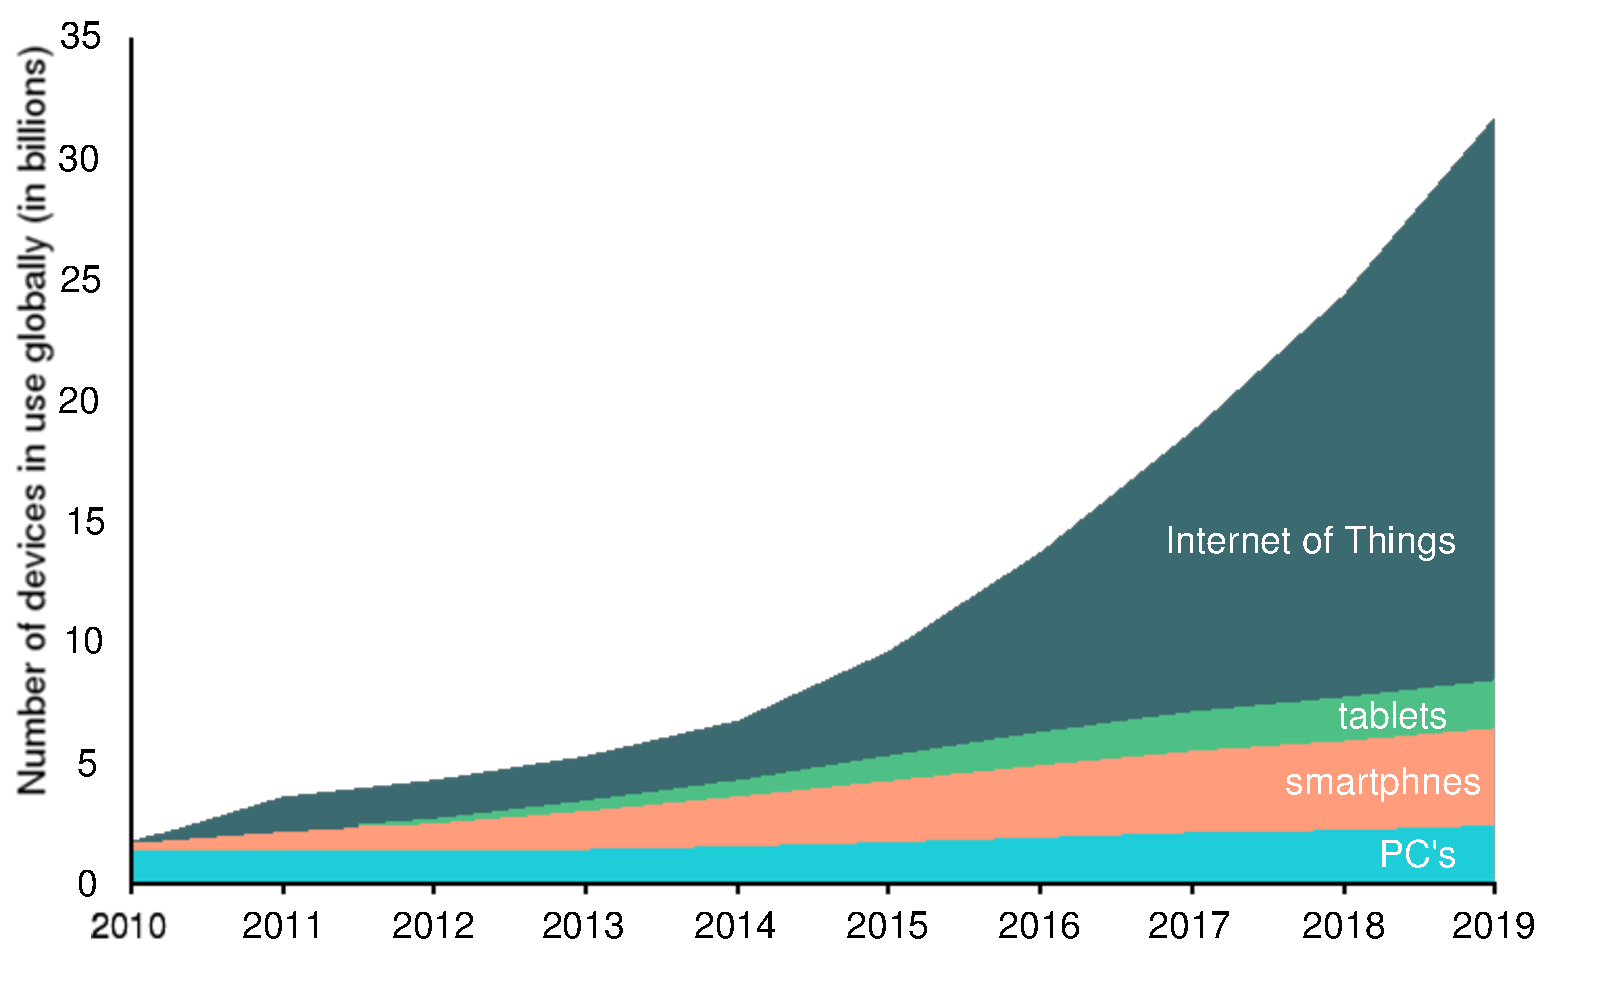
\includegraphics[width=10cm]{iot_devices}
\caption{Numero di dispositivi per anno}
\end{figure}

Questa rapida crescita ha portato alla ricerca è sviluppo di nuove soluzioni 
tecnologiche per supportare il carico di dispositivi simultaneamente connessi 
alla rete, senza avere un degrado evidente delle performance.
Per non alterare il \emph{QoS} Quality of Service della rete , hardware e
software dovranno essere rivisti insieme alla topologia di rete utilizzata. Alla
base di queste nuove tipologie di rete troviamo :

\begin{itemize}
\item \textbf{Scalabilità}: Dato l'elevato numero di devices connessi, scenari
urbani ed industriali, la network tecnologi alla base dovrà essere estremamente
adattabile, in maniera dinamica, al carico di dispositivi connessi.
\item \textbf{Costo unitario}: Il costo del singolo modulo, dovrà essere basso
per garantire la più ampia fetta di mercato.
\item \textbf{Durata della batteria}: La maggior parte dei dispositivi sarà
alimentata tramite batteria, e la durata minima cercata e pari a una decina d'anni. 
\item \textbf{Costo computazionale}: La modulazione alla base di queste nuove
tipologie di rete, dovrà essere concepita in modo da non avere un costo
computazionale elevato .
\item \textbf{Distanza}: La necessità di utilizzare questi devices in abmbienti
rurali, necessita devices in grado di inviare il messaggio per distanze di
alcuni chilometri.
\item \textbf{Sicurezza}: La comunicazione con il devices dovrà essere sicura e
ogni devices necessita la possibilità di aggiornamenti software
\item \textbf{Menagment}: I vari dispositivi dovranno essere facilmente
controllabili da remoto.
\item \textbf{Fail-safe}: Il mal  funzionamento di un  device non dovrà
compromettere l'intera infrastruttura a lui connessa. 
\end{itemize}

\begin{figure}[h]
\centering 
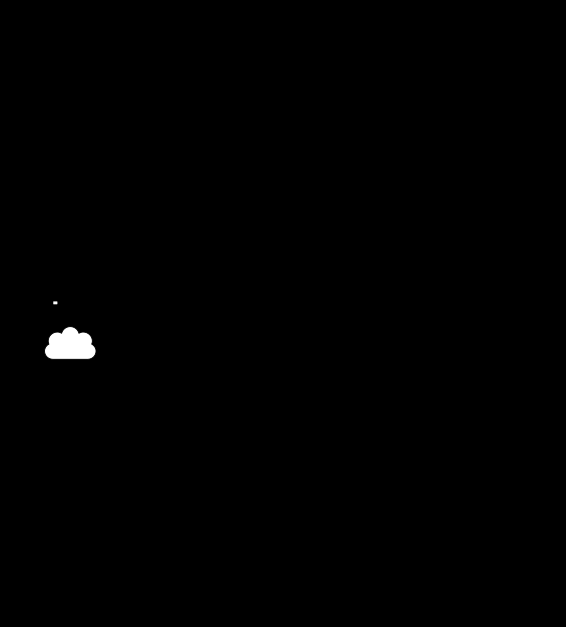
\includegraphics[width=10cm]{three-layer}
\caption{Layer del IoT}
\end{figure}

Vari tipi di architetture di rete sono stati proposti per realizzare questa
nuova infrastruttura. Per quanto le varie proposte si basano su tecnologie
differenti, è possibile individuare tre layer comuni 
\begin{itemize}
\item \textbf{Device layer} formato da tutti i dispositivi che collezionano dati
e sono connessi alla rete.
\item \textbf{Network layer} La struttura della rete, la quale permette di
connettere i vari devices in modo che possano scambiare i dati tra di loro o
inviarli ad un data-center.
\item \textbf{Application layer} il quale interpreta e utilizza i dati ricevuti.
\end{itemize}

Attualmente sono diversi i concorrenti che provano ad affermarsi nel settore
del IoT proponendo soluzioni diverse. Nei seguenti capitoli ci sarà un analisi
generale delle varie topologie proposte, in particolare verrà analizzata la
tecnologia Lora ed il protocolla LoraWAN.

